\documentclass[12pt]{article} 
\usepackage{amsmath}
\usepackage{amssymb}
\usepackage{pgf,tikz}
\usepackage{xcolor}
\usetikzlibrary{decorations.pathreplacing,arrows}
\usetikzlibrary{positioning,chains,fit,shapes,calc}
\tikzstyle{vertex}=[circle,draw=black,fill=black,inner sep=0,minimum size=3pt,text=white,font=\footnotesize]
\usetikzlibrary{graphs}
\usetikzlibrary{shapes.symbols}

\begin{document}

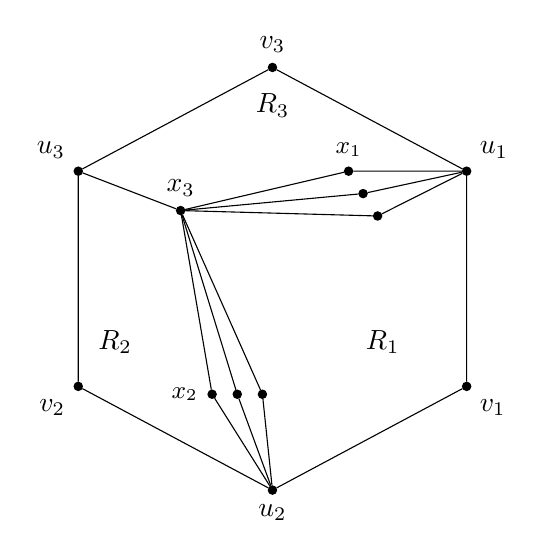
\begin{tikzpicture}
    \node[] (z){};
    \node[vertex, label=above right:$u_1$] (u1) [above right=1.2cm and 2.3cm of z] {};
    \node[vertex, label=below right:$v_1$] (v1) [below right=1.2cm and 2.3cm of z] {};
    \node[vertex, label=below:$u_2$] (u2) [below=2.5cm of z] {};
    \node[vertex, label=below left:$v_2$] (v2) [below left=1.2cm and 2.3cm of z] {};
    \node[vertex, label=above left:$u_3$] (u3) [above left=1.2cm and 2.3cm of z] {};
    \node[vertex, label=above:$v_3$] (v3) [above=2.5cm of z] {};


    \node[vertex, label=above:$x_3$] (x3) [above left=0.7cm and 1cm of z] {};

    \node[vertex, label=above: {\small $x_1$}] (x1) [above right= 1.2cm and 0.8cm of z]{};
    \node[vertex] (x12) [below right= 0.2cm and 0.1cm of x1]{};
    \node[vertex] (x13) [below right= 0.2cm and 0.1cm of x12]{};


    \node[vertex, label=left:{\small $x_2$}] (x2) [below left=1.3cm and 0.6cm of z] {};
    \node[vertex] (x22) [right=0.2cm of x2] {};
     \node[vertex] (x23) [right=0.2cm of x22] {};


     \node[] at (0,2.2) {$R_3$};
     \node[] at (1.4,-0.8) {$R_1$};
     \node[] at (-2,-0.8) {$R_2$};


    \draw (u1) -- (v1) -- (u2) -- (v2) -- (u3) -- (v3) -- (u1);
    \draw (u3) -- (x3);
    \draw (u1) -- (x1) -- (x3) -- (x2) -- (u2);
    \draw (u1) -- (x12) -- (x3) -- (x22) -- (u2);
    \draw (u1) -- (x13) -- (x3) -- (x23) -- (u2);
\end{tikzpicture}

\end{document}